\chapter{How the software works} \label{chap:eight}

This chapter aims to sum up everything discussed over the last several chapters and give an overview of how the software bundle presented in this article functions as a whole. Note that this chapter does not include instructions on how to run the software. For that, please refer to \autoref{chap:b} and its sections explaining how to do that step by step.

The process of running simulations and storing the obtained data is managed by the run.py script which delegates the tasks to other scripts until the simulation session is concluded. It is called by the \textbf{run.sh} script, which the user must use to start the simulation session. It takes the participant's name as an argument and an optional keyword,``ai", indicating that an AI implementation will drive the scenarios. The run.py script creates a directory for each participant in the data/recordings directory and, within it, creates a directory for each scenario in which the participant will participate. This approach allows for easy access and organisation of the recorded data during analysis.

The scenarios that the vehicle has to drive are listed in the carla\_scripts/scenario\_list.json file. An example of the scenario list file can be seen in \autoref{fig:scenario_list} in \autoref{chap:a}. Here all the scenarios that the participant is supposed to drive are shown. If the scenario or path is not specified (they are null), the algorithm will automatically generate them during run-time, resulting in a new and unseen route. 

For each scenario, a corresponding \textbf{scenario\_manager.py} script is launched that takes care of the scenario simulation process. It first generates a path and scenario if they are not specified, then changes the map and weather, populates the map, and defines the behaviour of actors on the road. In the beginning, all the simulation actors are immobilised to ensure that each simulation begins with the same conditions for each participant.

Once everything is set up, the hero vehicle is spawned. Depending on if the ``ai" keyword was specified when the run.sh script was launched, the scenario manager either launches a manually controlled vehicle or the self-driving one. For that, either driver.py (keyboard or steering wheel) or self\_driver.py scripts are called.

If a human driver controls the car, then once the Python application for driving is launched, the driver, in order to start the simulation, needs to press the BACKSPACE key. This causes the Scenario to unfreeze all actors in the simulation, allowing them to move around the world according to their designated behaviour. The simulation also launches the Manager module responsible for all performance calculations and violation marking.

The simulation can end in two ways: reaching the finish line or pressing the BACKSPACE key to abort the simulation. The latter option was added to allow immediate simulation termination if something goes wrong and make it easy to rerun the simulation later (thanks to the flexible structure). Once the simulation finishes, all data and the simulation recording are saved to disk, and the subsequent simulation is launched. The process is repeated until all the scenarios have run from the scenario\_list.json file. Note that manual driving can be done either using a keyboard or a steering wheel. The type used can be changed by uncommenting line 158 or line 157 in software/carla\_scripts/simulation\_manager.py script.

If the AV implementation is driving in the scenarios, everything is happening automatically, and no buttons need to be pressed. Only the run.sh script needs to be run with the participant's name and the keyword ``ai".

The simulation process is also illustrated in \autoref{fig:simulation_process}, providing a visual overview of how the components act together.

\begin{figure}
    \centering
    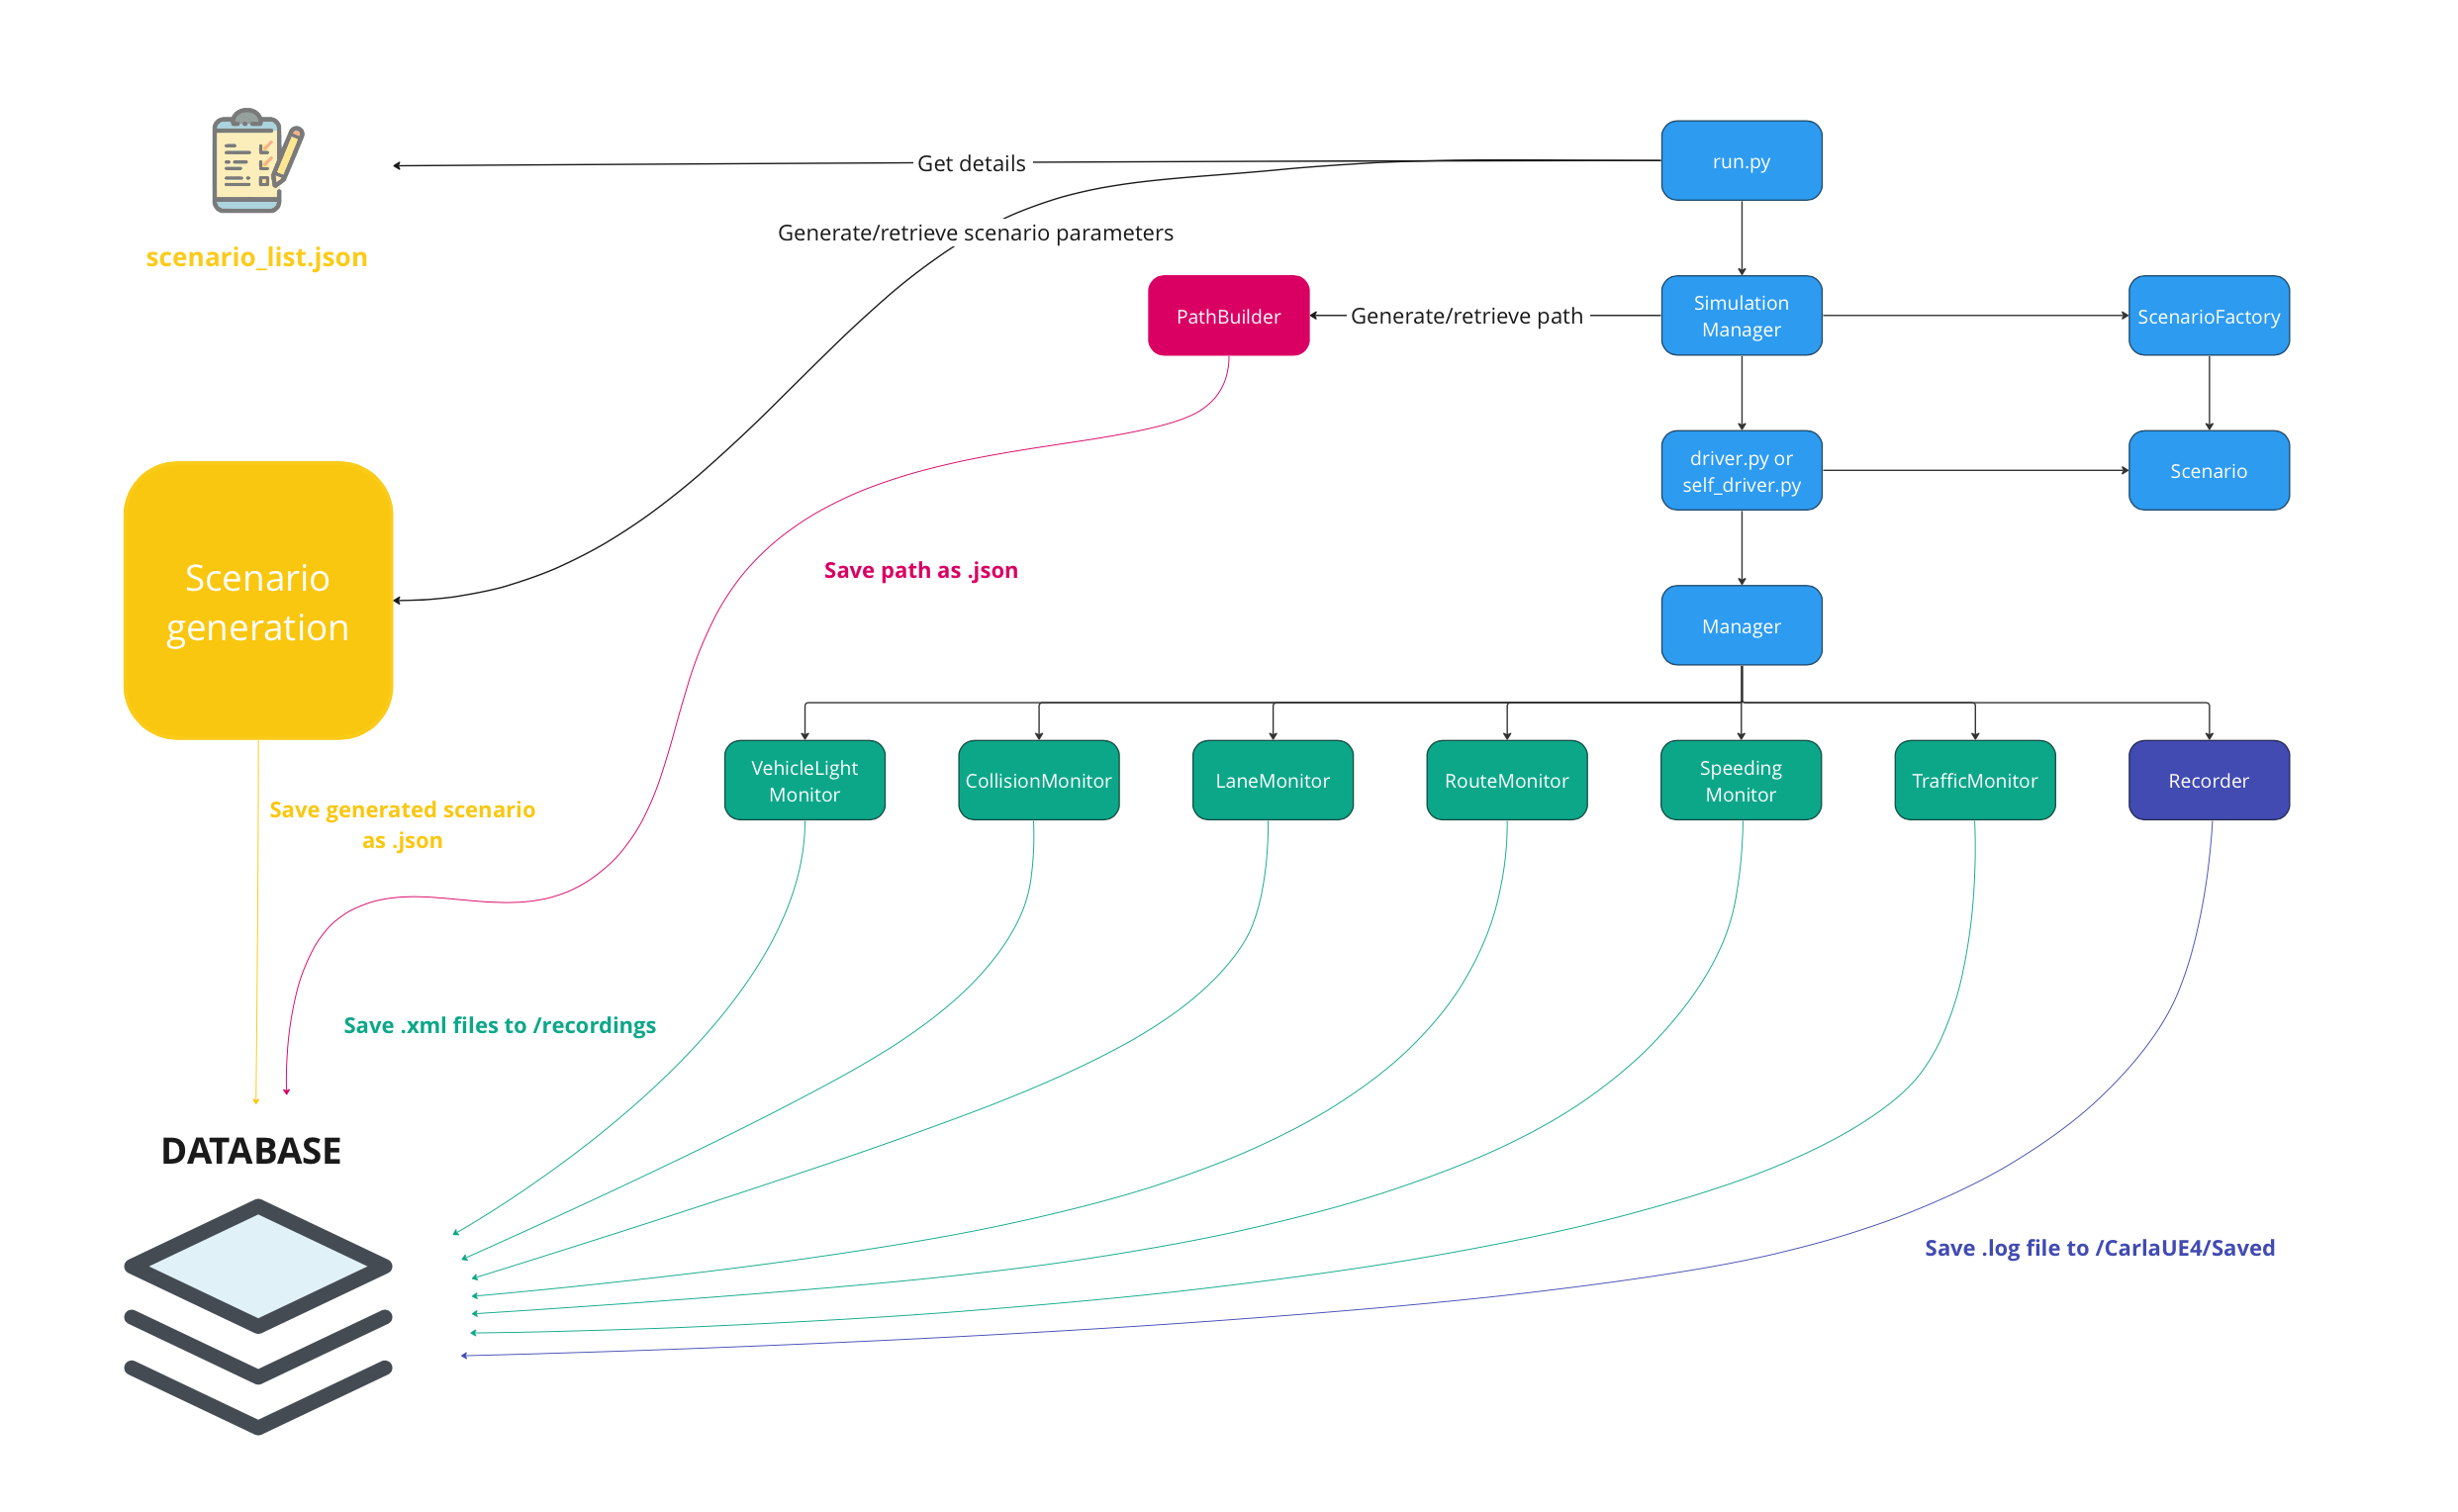
\includegraphics[width = \textwidth]{research_paper/Images/simulation_process.png}
    \caption{An overview of the simulation process}
    \label{fig:simulation_process}
\end{figure}

It is crucial to mention that not only the CARLA agent can drive in the simulations but any AV implementation that can be bridged with the CARLA simulator. After the connection to the simulator is complete, all that is needed is to give the waypoints generated by the GlobalRoutePlanner to the agent to follow, name the vehicle ``hero" within the simulated environment and start the Manager module when the simulation starts and terminate it once the finish is reached. Everything else works independently, talking to the server directly and receiving the necessary information.

Once the simulations are complete, the user can run the analysis and then work with the analysed data. More about how to use all the software elements can be found in \autoref{chap:b}.

Several additional Python scripts were written to understand the CARLA world better and help design the scenarios. These include print\_coordinates.py, which prints the precise coordinates of the spectator, who can fly anywhere in the world, and draw\_lanes\_terminal.py, which generates a route when given start and finish coordinates and marks all legal lanes on the map. Other useful scripts can be found in the sub-directories of the software/carla\_script directory.

One necessary script to mention is the replay.sh, which enables the replay of any simulation driven by a specific participant on the screen. For example, by executing the command ``/replay.sh participant\_A 1" in the terminal, the simulation of the first scenario driven by participant\_A will be replayed.